%-------------------------------------------------------------------------------
% LATEX TEMPLATE - CONCEPT-AWARE GEOLOCATION REPORT
%-------------------------------------------------------------------------------

\documentclass{uva-inf-article}
\usepackage[english]{babel}
\usepackage{amsmath, amssymb, amsfonts}
\usepackage{booktabs}
\usepackage{tabularx}
\usepackage{array}
\usepackage{algorithm}
\usepackage{algorithmic}
\usepackage{graphicx}
\usepackage{subcaption}
\usepackage{multirow}
\usepackage{xcolor}

\usepackage[style=authoryear-comp]{biblatex}
\addbibresource{references.bib}

%-------------------------------------------------------------------------------
%	DOCUMENT METADATA
%-------------------------------------------------------------------------------

\title{Concept-Aware Geolocation with Hierarchical Concept Bottleneck Models}

\assignment{Project AI}

\authors{Pradyut Nair}
\uvanetids{15558169}

\mentor{Nanne van Noord}
\docent{}

%\group{AI Research Group}

\date{\today}

%-------------------------------------------------------------------------------
%	DOCUMENT CONTENT
%-------------------------------------------------------------------------------

\begin{document}
\maketitle

\tableofcontents
\begin{abstract}
Image geolocation, the task of predicting geographic coordinates from visual input, remains challenging due to the inherent ambiguity of similar-looking scenes across different regions. While existing approaches achieve reasonable accuracy through end-to-end learning, they operate as black boxes, providing little insight into \textit{why} a particular location is predicted. This work presents a Concept-Aware Geolocation system that learns interpretable semantic concepts as an intermediate representation for location prediction. We propose a three-stage curriculum learning pipeline combining domain-specific contrastive pretraining, hierarchical text-anchored concept learning, and cross-attention-based geolocation. Our architecture enforces a strict concept bottleneck, ensuring all predictions flow through human-interpretable semantic concepts. Experiments on a 43,000-image street view dataset demonstrate that our approach achieves a median error of 126 km on in-distribution data and 350 km on out-of-distribution GeoGuessr images, while providing patch-level attention maps that reveal which visual regions support concept-based predictions.
\end{abstract}

%-------------------------------------------------------------------------------
%	INTRODUCTION
%-------------------------------------------------------------------------------

\section{Introduction}
\label{sec:introduction}

Visual geolocation has emerged as an important capability for applications ranging from autonomous navigation and urban planning to content verification and disaster response \parencite{hays2008im2gps}. The fundamental challenge lies in inferring precise geographic coordinates from images that may contain ambiguous or region-agnostic visual patterns. A rural road in Argentina may appear remarkably similar to one in Australia, while distinctive architectural styles or vegetation patterns can provide strong localization cues that humans intuitively recognize.

Early approaches to image geolocation treated the problem as scene retrieval, matching query images against geo-tagged reference databases \parencite{hays2008im2gps}. The seminal PlaNet model \parencite{weyand2016planet} reformulated geolocation as classification over discrete geographic cells, demonstrating that convolutional neural networks could learn globally discriminative visual features. Subsequent work improved accuracy through hierarchical cell structures \parencite{muller2018geolocation, seo2018cpl} and multi-task learning, culminating in recent systems like PIGEON \parencite{haas2024pigeon} that achieve expert-level performance on GeoGuessr challenges.

However, these approaches share a critical limitation: they operate as opaque end-to-end systems that provide no insight into the reasoning behind predictions. This lack of interpretability poses significant challenges for safety-critical applications where understanding \textit{why} a location was predicted is as important as the prediction itself. Furthermore, without explicit semantic reasoning, models may learn spurious correlations (such as watermarks or camera artifacts) rather than meaningful geographic indicators.

Recent advances in vision-language models, particularly CLIP \parencite{radford2021learning} and its geographic variants like StreetCLIP \parencite{streetclip2023} and GeoCLIP \parencite{cepeda2023geoclip}, have demonstrated powerful capabilities for aligning visual and textual representations. These models learn to understand semantic concepts and their relationships to visual patterns through contrastive learning on large-scale image-text pairs. Concept Bottleneck Models (CBMs) \parencite{koh2020concept} provide a framework for interpretable prediction by forcing all decisions to flow through an intermediate layer of human-understandable concepts.

This work combines these advances to develop a concept-aware geolocation system that predicts locations through explicit semantic reasoning. Our approach offers three key advantages over traditional end-to-end methods. First, by requiring predictions to flow through a concept bottleneck, we ensure that the model's reasoning can be inspected and understood. Second, learning explicit concepts enables generalization to novel locations that share semantic characteristics with training data. Third, cross-attention mechanisms provide patch-level explanations showing which image regions support specific concept activations.

We make the following contributions:
\begin{itemize}
    \item A hierarchical concept bottleneck architecture with two levels of semantic abstraction (fine-grained child concepts and coarse parent concepts) and consistency losses enforcing their relationships.
    
    \item A text-anchored prototype learning approach where concept representations are initialized from CLIP text embeddings and adapted through learnable residuals, maintaining semantic grounding while enabling visual specialization.
    
    \item A cross-attention geolocation module where concept embeddings query image patch tokens, providing interpretable spatial attention maps alongside coordinate predictions.
    
    \item Adaptive semantic geocells generated through per-country clustering that allocate prediction granularity according to regional data density.
\end{itemize}

%-------------------------------------------------------------------------------
%	RELATED WORK
%-------------------------------------------------------------------------------

\section{Related Work}
\label{sec:related}

Visual geolocation research has evolved from retrieval-based methods \parencite{hays2008im2gps} to classification over geographic partitions. PlaNet \parencite{weyand2016planet} demonstrated that training CNNs to classify images into approximately 26,000 S2 cells could achieve reasonable global geolocation. Hierarchical approaches \parencite{muller2018geolocation} improved performance by predicting at multiple spatial scales, while CPlaNet \parencite{seo2018cpl} introduced combinatorial partitioning for finer-grained predictions. Recent work leverages large-scale pretraining: StreetCLIP \parencite{streetclip2023} fine-tunes CLIP on street view imagery, and GeoCLIP \parencite{cepeda2023geoclip} learns joint embeddings of images and GPS coordinates through contrastive learning.

The concept bottleneck framework \parencite{koh2020concept} addresses neural network interpretability by inserting a layer of human-understandable concepts between input features and final predictions. This design ensures that all model decisions can be traced to specific concept activations, enabling both interpretation and intervention. Extensions have explored concept learning from language supervision, hierarchical concept structures, and applications beyond classification to regression and generation.

CLIP \parencite{radford2021learning} learns aligned vision-language representations through contrastive learning on 400 million image-text pairs. This foundation enables zero-shot transfer to novel visual concepts through natural language descriptions. GeoCLIP \parencite{cepeda2023geoclip} extends this paradigm to geographic understanding by training a location encoder alongside CLIP's image encoder, learning joint embeddings where visually similar locations cluster together. Our work builds on these foundations by introducing an explicit concept bottleneck that mediates between visual features and geographic predictions.

%-------------------------------------------------------------------------------
%	METHODOLOGY
%-------------------------------------------------------------------------------

\section{Methodology}
\label{sec:methodology}

Our approach follows a curriculum learning strategy \parencite{bengio2009curriculum} that progressively builds a concept-aware geolocation system through three training stages. This staged approach allows each component to specialize before being integrated into the complete system, preventing optimization conflicts between different learning objectives.

\begin{figure}[h!]
    \centering
    \includegraphics[width=\textwidth]{arch3.png}
    \caption{Three-stage architecture for concept-aware geolocation. Stage 0 performs domain contrastive pretraining to align image, GPS, and concept embeddings. Stage 1 learns hierarchical concept classification through text-anchored prototypes. Stage 2 predicts geographic coordinates via cross-attention between concept embeddings and image patches.}
    \label{fig:architecture}
\end{figure}

\subsection{Dataset and Preprocessing}

We utilize a dataset of 43,040 street view panorama images collected from diverse geographic locations. Each sample contains an image, GPS coordinates (latitude and longitude), a child concept label describing the fine-grained scene type (e.g., ``Urban Street'', ``Suburban Road'', ``Rural Landscape''), a parent concept providing coarse categorization (e.g., ``Urban'', ``Rural'', ``Natural''), and the country of origin.

The dataset exhibits a hierarchical concept structure with approximately 100 child concepts organized under 15 parent concepts. This hierarchy captures semantic relationships: for instance, child concepts ``Urban Street'', ``Commercial District'', and ``Residential Area'' all map to the parent concept ``Urban''. We leverage this hierarchy through consistency losses that encourage predictions at both levels to align.

Data is split into training (70\%), validation (15\%), and test (15\%) sets using stratified sampling by child concept to ensure all concepts appear in training. The same splits are used across all training stages for fair comparison.

\subsection{Semantic Geocell Generation}

Traditional approaches partition the Earth's surface uniformly, but this fails to account for non-uniform data distribution. Urban areas contain far more street view imagery than remote regions. We address this through adaptive per-country clustering that allocates geocells according to regional data density.

For each country with sufficient samples, we convert GPS coordinates to 3D Cartesian positions on the unit sphere and apply K-means clustering with $k = \lceil n / s \rceil$ clusters, where $n$ is the sample count and $s = 500$ is the minimum samples per cell. Countries with fewer samples receive a single cell at their centroid. This process produces 1,048 semantic geocells globally, with dense regions (Europe, North America, East Asia) receiving finer granularity than sparse regions.

Figure~\ref{fig:geocells} visualizes the resulting tessellation, showing how cell density adapts to data availability. The Voronoi diagram illustrates coverage, while the latitude distribution confirms concentration in populated northern hemisphere regions.

\begin{figure}[h!]
    \centering
    \begin{subfigure}[b]{0.48\textwidth}
        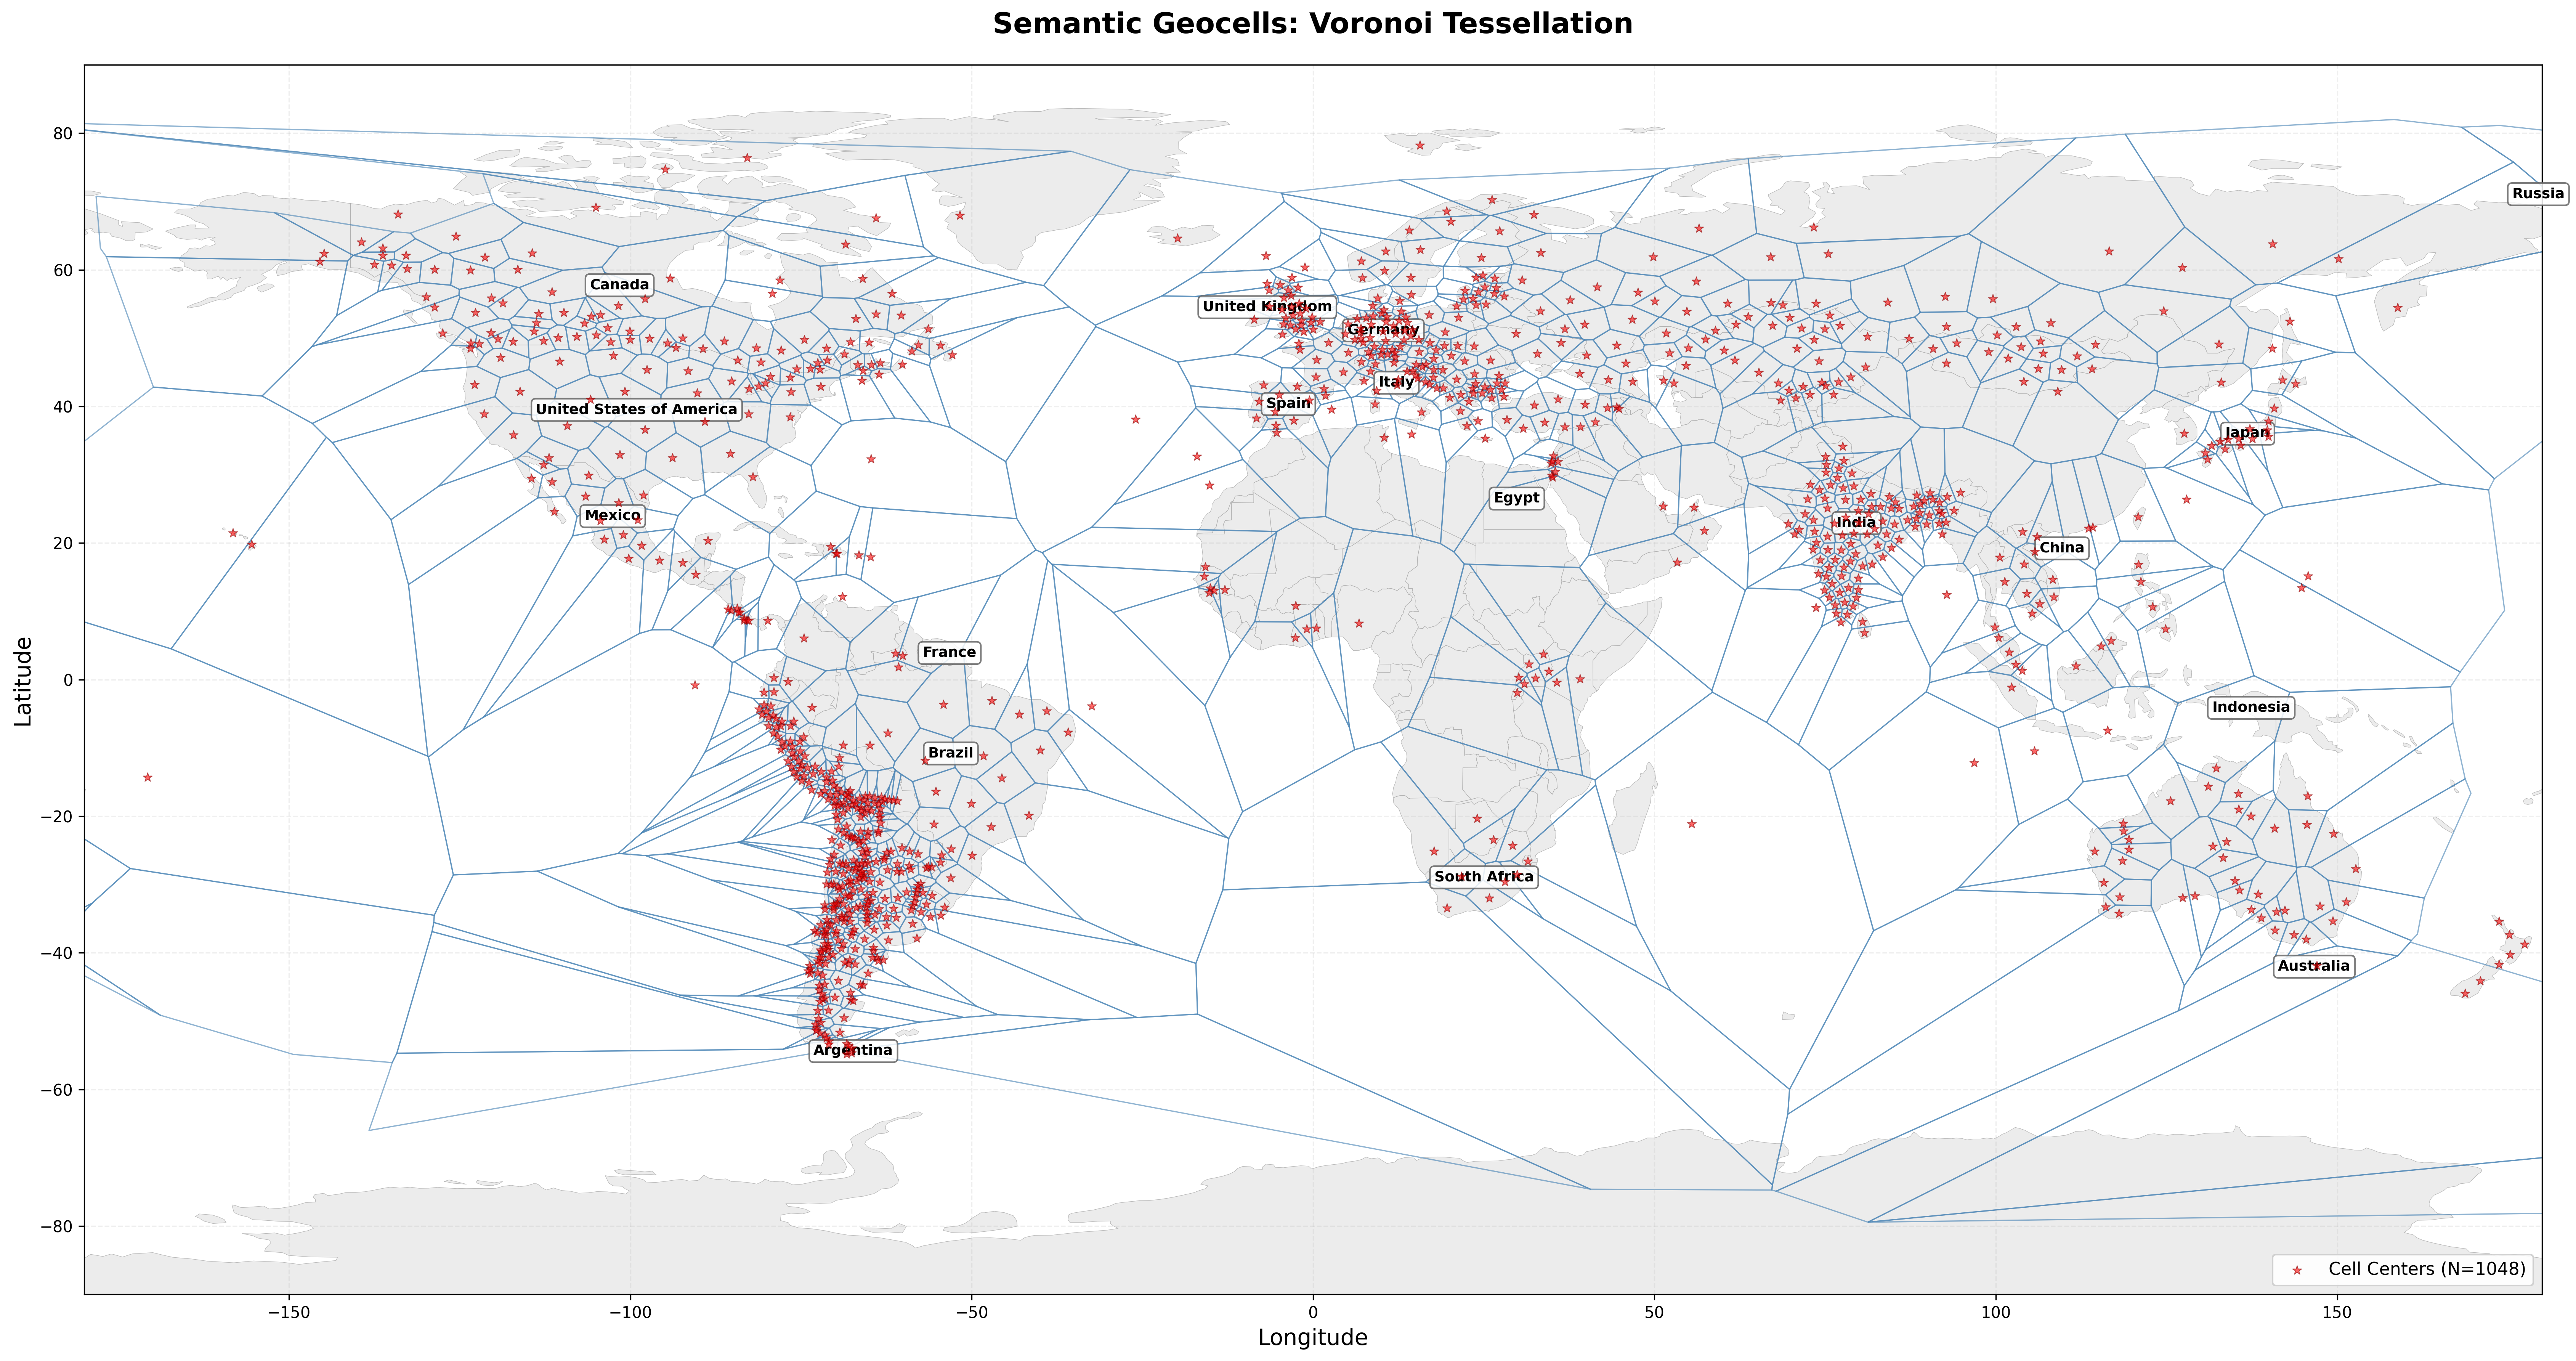
\includegraphics[width=\textwidth]{geocells_map/geocells_map_finetuned_both.png}
        \caption{Voronoi tessellation of semantic geocells showing cell centers (red markers) and their boundaries. Cell density adapts to regional data availability.}
        \label{fig:geocells_map}
    \end{subfigure}
    \hfill
    \begin{subfigure}[b]{0.48\textwidth}
        \includegraphics[width=\textwidth]{geocells_map/cell_distribution_finetuned_both.png}
        \caption{Distribution of geocells by latitude (left) and hemisphere (right), showing concentration in northern populated regions.}
        \label{fig:geocells_dist}
    \end{subfigure}
    \caption{Adaptive semantic geocell generation through per-country K-means clustering in 3D Cartesian space. The 1,048 geocells provide finer granularity in data-dense regions while maintaining global coverage.}
    \label{fig:geocells}
\end{figure}

\subsection{Stage 0: Domain Contrastive Pretraining}

The first training stage adapts the StreetCLIP vision encoder to our specific domain through multi-objective contrastive learning. While StreetCLIP provides strong geographic priors from pretraining on street view imagery, we find that partial fine-tuning improves downstream concept learning and geolocation accuracy.

We unfreeze the top two transformer layers of the vision encoder while keeping lower layers frozen to preserve general visual representations. The model learns to align image embeddings with GPS coordinates, child concept prototypes, and parent concept prototypes through separate contrastive losses.

The core alignment objective uses InfoNCE loss \parencite{oord2018infonce} to bring image embeddings closer to their corresponding GPS embeddings while pushing apart embeddings from different locations:
\begin{equation}
\mathcal{L}_{\text{GPS}} = -\frac{1}{B}\sum_{i=1}^{B}\log\frac{\exp(\text{sim}(x_i, g_i)/\tau)}{\sum_{j=1}^{B}\exp(\text{sim}(x_i, g_j)/\tau)}
\end{equation}
where $x_i$ is the image embedding, $g_i$ is the GPS embedding from the GeoCLIP location encoder \parencite{cepeda2023geoclip}, and $\tau = 0.07$ is the temperature parameter.

Concept alignment losses similarly encourage image embeddings to cluster according to their semantic labels:
\begin{align}
\mathcal{L}_{\text{child}} &= \text{InfoNCE}(z, T_{\text{child}}, c_{\text{child}}, \tau) \\
\mathcal{L}_{\text{parent}} &= \text{InfoNCE}(z, T_{\text{parent}}, c_{\text{parent}}, \tau)
\end{align}
where $z$ is the concept embedding, $T_{\text{child}}$ and $T_{\text{parent}}$ are text-encoded prototype matrices, and $c_{\text{child}}$, $c_{\text{parent}}$ are the ground truth concept indices.

A hierarchy consistency loss encourages embeddings from the same parent category to cluster together in the concept space, enforcing the semantic relationship between child and parent concepts. An optional anchor loss prevents catastrophic forgetting by penalizing large deviations from the original StreetCLIP representations.

The total Stage 0 loss combines these objectives with learned weights:
\begin{equation}
\mathcal{L}_0 = \lambda_1\mathcal{L}_{\text{GPS}} + \lambda_2\mathcal{L}_{\text{child}} + \lambda_3\mathcal{L}_{\text{parent}} + \lambda_4\mathcal{L}_{\text{hierarchy}} + \lambda_5\mathcal{L}_{\text{patch}}
\end{equation}

Stage 0 trains for 20 epochs with batch size 128, using differential learning rates: $3 \times 10^{-5}$ for encoder layers and $1 \times 10^{-4}$ for projection heads.

\subsection{Stage 1: Text-Prototype Concept Learning}

The second stage learns concept representations through text-anchored classification with hierarchical supervision. The image encoder is frozen to preserve domain alignment from Stage 0, focusing learning on the concept bottleneck.

Rather than learning concept prototypes from scratch, we initialize them from CLIP text embeddings of concept descriptions. This provides strong semantic grounding: the prototype for ``Urban Street'' begins close to CLIP's representation of that phrase. We then add learnable residual vectors that allow adaptation to visual patterns specific to our street view domain:
\begin{equation}
T_{\text{child}} = \text{normalize}(\text{proj}(T^{\text{base}}_{\text{child}} + \Delta_{\text{child}}))
\end{equation}
where $T^{\text{base}}$ contains frozen text embeddings and $\Delta$ is a learnable residual initialized from $\mathcal{N}(0, 0.01)$. The projection maps from the 768-dimensional CLIP space to our 512-dimensional concept embedding space.

Concept predictions are computed through cosine similarity to prototypes with learned temperature and bias terms:
\begin{align}
\text{logits}_{\text{child}} &= s_{\text{child}} \cdot (z \cdot T_{\text{child}}^T) + b_{\text{child}} \\
\text{logits}_{\text{parent}} &= s_{\text{parent}} \cdot (z \cdot T_{\text{parent}}^T) + b_{\text{parent}}
\end{align}
where $s$ are learnable temperature scales (initialized to 14.0) and $b$ are per-class bias terms.

Stage 1 employs focal loss \parencite{lin2017focal} for classification to address class imbalance, with label smoothing of 0.2 for regularization:
\begin{equation}
\mathcal{L}_{\text{focal}} = -\alpha(1-p_t)^\gamma \log(p_t)
\end{equation}
where $\gamma = 2.0$ controls the focus on hard examples.

A hierarchical consistency loss ensures that child predictions aggregate correctly to parent predictions through KL divergence between the expected and predicted parent distributions:
\begin{equation}
\mathcal{L}_{\text{consistency}} = \text{KL}(\text{softmax}(\text{logits}_{\text{child}}) \cdot M_{\text{hier}} \| \text{softmax}(\text{logits}_{\text{parent}}))
\end{equation}
where $M_{\text{hier}} \in \mathbb{R}^{k_c \times k_p}$ is the child-to-parent mapping matrix.

Additional losses include inter-parent contrastive learning (pushing apart embeddings from different parent categories), prototype contrastive alignment (encouraging embeddings to match their assigned prototypes), L2 regularization on learnable residuals, and intra-parent consistency (encouraging child prototypes within the same parent to remain similar).

Stage 1 trains for 50 epochs with batch size 256 using precomputed image embeddings for efficiency, learning rate $3 \times 10^{-4}$, and AdamW optimizer \parencite{loshchilov2017adamw}.

\subsection{Stage 2: Cross-Attention Geolocation}

The final stage predicts geographic coordinates through cross-attention between concept embeddings and image patch tokens. This design maintains the concept bottleneck constraint while leveraging fine-grained spatial information.

The Stage 2 model receives frozen concept embeddings $z \in \mathbb{R}^{512}$ from Stage 1 and frozen patch tokens $P \in \mathbb{R}^{576 \times 1024}$ from the image encoder. Patch tokens are projected to the concept embedding dimension, then a multi-head cross-attention mechanism \parencite{vaswani2017attention} allows concept queries to attend over spatial positions:
\begin{align}
Q &= W_Q \cdot z \in \mathbb{R}^{1 \times 512} \\
K &= W_K \cdot P_{\text{proj}} \in \mathbb{R}^{576 \times 512} \\
V &= W_V \cdot P_{\text{proj}} \in \mathbb{R}^{576 \times 512} \\
\text{attn} &= \text{softmax}(QK^T / \sqrt{d}) \cdot V
\end{align}

The attention weights $\alpha \in \mathbb{R}^{576}$ can be reshaped to a $24 \times 24$ spatial map, providing interpretable visualization of which image regions most strongly support the concept-based prediction.

The attention output is combined with the original concept embedding through residual connection and layer normalization \parencite{ba2016layer}:
\begin{equation}
z' = \text{LayerNorm}(z + \text{attn})
\end{equation}
followed by a feed-forward network with another residual connection.

Two prediction heads operate on the fused representation. A cell classification head predicts the geocell membership through softmax over 1,048 classes. An offset regression head predicts the 3D Cartesian offset from the predicted cell center to the actual location.

To understand component contributions, we implement three inference modes:
\begin{itemize}
    \item \textbf{Both}: Full cross-attention fusion of concepts and patches (default)
    \item \textbf{Concept-only}: Predictions from concept embedding alone, bypassing cross-attention
    \item \textbf{Image-only}: Predictions from pooled patch tokens, bypassing the concept bottleneck
\end{itemize}

The total Stage 2 loss combines cell classification cross-entropy and offset regression MSE:
\begin{equation}
\mathcal{L}_2 = \mathcal{L}_{\text{cell}} + \lambda_{\text{offset}}\mathcal{L}_{\text{offset}}
\end{equation}
with $\lambda_{\text{offset}} = 5.0$.

Stage 2 trains for 30 epochs with batch size 32, learning rate $1 \times 10^{-4}$. Final coordinates are computed as the predicted cell center plus the regressed offset, converted from Cartesian to latitude/longitude.

%-------------------------------------------------------------------------------
%	EXPERIMENTS
%-------------------------------------------------------------------------------

\section{Experiments}
\label{sec:experiments}

We evaluate our approach on both in-distribution test data and an out-of-distribution GeoGuessr dataset to assess generalization. All experiments compare two model variants: \textbf{vanilla} (Stage 1 and 2 only, without Stage 0 pretraining) and \textbf{finetuned} (complete three-stage pipeline with Stage 0 pretraining).

\subsection{Evaluation Metrics}

For concept classification (Stage 1), we report top-1 and top-5 accuracy for both child and parent concepts. For geolocation (Stage 2), we report median and mean haversine distance error in kilometers, geocell classification accuracy, and threshold accuracies at standard geographic scales:
\begin{itemize}
    \item \textbf{Street}: within 1 km
    \item \textbf{City}: within 25 km
    \item \textbf{Region}: within 200 km
    \item \textbf{Country}: within 750 km
\end{itemize}

\subsection{Stage 1: Concept Classification Results}

Table~\ref{tab:stage1} presents concept classification results on the held-out test set (4,304 samples).

\begin{table}[h!]
\centering
\begin{tabularx}{\columnwidth}{l*{4}{>{\centering\arraybackslash}X}}
\toprule
\textbf{Variant} & \textbf{Child (Top-1)} & \textbf{Parent (Top-1)} & \textbf{Child (Top-5)} & \textbf{Parent (Top-5)} \\
\midrule
Vanilla & 0.455 & 0.386 & 0.681 & 0.713 \\
Finetuned & \textbf{0.461} & \textbf{0.480} & \textbf{0.716} & \textbf{0.725} \\
\bottomrule
\end{tabularx}
\caption{Stage 1 concept classification accuracy on the test split. The finetuned variant with Stage 0 pretraining shows improved parent concept accuracy, indicating better hierarchical structure learning.}
\label{tab:stage1}
\end{table}

Both variants achieve comparable child concept accuracy around 46\%, reflecting the challenge of distinguishing among approximately 100 fine-grained categories. The finetuned variant shows notably improved parent concept accuracy (48.0\% vs 38.6\%), suggesting that Stage 0 pretraining helps learn the hierarchical concept structure. Top-5 accuracies exceed 70\% for both levels, indicating that the correct concept typically ranks highly even when not the top prediction.

Accuracy varies substantially across concepts, with common categories like ``Urban Street'' achieving higher accuracy than rare categories due to training data distribution.

\subsection{Stage 2: Geolocation Results}

Table~\ref{tab:stage2_test} presents geolocation results on the test split, comparing ablation modes and model variants.

\begin{table}[h!]
\centering
\small
\begin{tabularx}{\columnwidth}{l>{\raggedright\arraybackslash}X*{6}{>{\centering\arraybackslash}X}}
\toprule
\textbf{Variant} & \textbf{Mode} & \textbf{Median (km)} & \textbf{Mean (km)} & \textbf{Cell Acc} & \textbf{City} & \textbf{Region} & \textbf{Country} \\
\midrule
\multirow{3}{*}{Vanilla} 
& Both & 133.2 & 713.8 & 0.454 & 0.215 & 0.574 & 0.830 \\
& Concept & 139.0 & 745.9 & 0.451 & 0.195 & 0.566 & 0.824 \\
& Image & 222.0 & 1070.5 & 0.374 & 0.175 & 0.482 & 0.753 \\
\midrule
\multirow{3}{*}{Finetuned} 
& Both & \textbf{126.0} & \textbf{684.6} & \textbf{0.449} & \textbf{0.232} & \textbf{0.578} & \textbf{0.829} \\
& Concept & 137.0 & 688.6 & 0.443 & 0.227 & 0.564 & 0.822 \\
& Image & 154.0 & 790.5 & 0.430 & 0.202 & 0.546 & 0.806 \\
\bottomrule
\end{tabularx}
\caption{Stage 2 geolocation performance on the in-distribution test split. The finetuned variant with full cross-attention (``both'') achieves the best median error of 126 km.}
\label{tab:stage2_test}
\end{table}

The results reveal several key patterns. Across all ablation modes, the finetuned variant consistently outperforms vanilla, with the best configuration achieving 126 km median error compared to 133 km for vanilla. This uniform advantage demonstrates that Stage 0 pretraining provides broadly beneficial representations regardless of inference configuration.

Within each variant, comparing different modes shows that concept-only predictions closely approach full model performance. For finetuned, concept-only achieves 137.0 km versus 126.0 km for the full model, validating our core interpretability goal that predictions can be understood through concept activations without significant accuracy sacrifice. In contrast, image-only mode performs notably worse (154.0 km for finetuned, 222.0 km for vanilla), indicating that the concept bottleneck provides regularization benefits beyond interpretability by preventing overfitting to low-level visual patterns.

Despite variation in fine-grained accuracy, country-level accuracy exceeds 80\% across all configurations, showing that the models maintain reliable coarse localization even when precise predictions are uncertain.


\subsection{Out-of-Distribution Evaluation}
To assess generalization, we evaluate on an external GeoGuessr dataset containing 5,477 images not seen during training. Table~\ref{tab:stage2_hf} presents these results.

\begin{table}[h!]
\centering
\small
\begin{tabularx}{\columnwidth}{l>{\raggedright\arraybackslash}X*{6}{>{\centering\arraybackslash}X}}
\toprule
\textbf{Variant} & \textbf{Mode} & \textbf{Median (km)} & \textbf{Mean (km)} & \textbf{Cell Acc} & \textbf{City} & \textbf{Region} & \textbf{Country} \\
\midrule
\multirow{3}{*}{Vanilla} 
& Both & 391.5 & 1643.7 & 0.234 & 0.032 & 0.323 & 0.673 \\
& Concept & 417.6 & 1788.8 & 0.222 & 0.033 & 0.310 & 0.644 \\
& Image & 448.4 & 1894.7 & 0.217 & 0.026 & 0.301 & 0.631 \\
\midrule
\multirow{3}{*}{Finetuned} 
& Both & \textbf{349.9} & \textbf{1616.9} & \textbf{0.265} & \textbf{0.034} & \textbf{0.360} & \textbf{0.688} \\
& Concept & 381.8 & 1670.2 & 0.255 & 0.032 & 0.340 & 0.665 \\
& Image & 387.0 & 1709.8 & 0.242 & 0.030 & 0.336 & 0.665 \\
\midrule
GeoCLIP & -- & 1015.8 & 3190.6 & -- & 0.027 & 0.160 & 0.424 \\
\bottomrule
\end{tabularx}
\caption{Stage 2 geolocation performance on the out-of-distribution GeoGuessr dataset. Performance degrades compared to in-distribution data, with the finetuned variant showing better generalization.}
\label{tab:stage2_hf}
\end{table}

Out-of-distribution performance reveals the generalization capabilities of our approach. Median error increases substantially compared to in-distribution results, reflecting the expected distribution shift between training and GeoGuessr imagery. Despite this challenge, the finetuned variant maintains superior performance across all evaluation metrics, with the best configuration achieving 349.9 km median error compared to 391.5 km for vanilla.

Comparing variants within each ablation mode confirms the consistent benefit of Stage 0 pretraining. The finetuned model achieves lower median error than vanilla for all three modes, with improvements ranging from approximately 9 to 14\% depending on the configuration. This uniform advantage validates that Stage 0 pretraining provides broadly transferable representations regardless of inference configuration.

Even with the distribution shift, country-level accuracy remains above 63\% across all configurations, indicating robust coarse localization. The baseline GeoCLIP model achieves significantly higher median error (1015.8 km) and lower threshold accuracies across all scales, demonstrating the advantage of our concept-aware approach even for out-of-distribution data.
Figure~\ref{fig:stage2_results} visualizes performance across ablation modes and evaluation settings.

\begin{figure}[h!]
    \centering
    \begin{subfigure}[b]{0.48\textwidth}
        \includegraphics[width=\textwidth]{analysis/stage2_test_split_results.png}
        \caption{In-distribution test split performance}
        \label{fig:stage2_test}
    \end{subfigure}
    \hfill
    \begin{subfigure}[b]{0.48\textwidth}
        \includegraphics[width=\textwidth]{analysis/stage2_hf_results.png}
        \caption{Out-of-distribution GeoGuessr performance}
        \label{fig:stage2_hf}
    \end{subfigure}
    \caption{Stage 2 geolocation results comparing model variants and ablation modes. The finetuned variant excels on both in-distribution and out-of-distribution data, demonstrating the value of Stage 0 pretraining for generalization.}
    \label{fig:stage2_results}
\end{figure}

% \subsection{Ablation Analysis}

% A comparative analysis of the three ablation modes reveals the value of different model components. For the finetuned variant on the in-distribution test split (Table~\ref{tab:stage2_test}), the ``both'' configuration achieves the best performance (126.0 km), with concept-only closely following (137.0 km, only 8.7\% worse), indicating that the concept bottleneck captures most of the predictive signal. Image-only performs notably worse (154.0 km), suggesting that semantic concepts provide better regularization than raw visual features.

% On the out-of-distribution GeoGuessr dataset (Table~\ref{tab:stage2_hf}), the finetuned ``both'' mode again leads (349.9 km), but concept-only falls further behind (381.8 km, 9.1\% worse). This widening gap indicates that spatial attention through cross-attention provides critical regularization for generalization to novel imagery. Image-only remains the weakest performer (387.0 km). Comparing across variants, finetuned consistently outperforms vanilla for all three modes, confirming the broad value of Stage 0 pretraining.

% \begin{figure}[h!]
%     \centering
%     \includegraphics[width=\textwidth]{analysis/stage2_finetuned_radar.png}
%     \caption{Ablation analysis for the finetuned model variant. The ``both'' mode (combining concepts and cross-attention) achieves the best overall performance, but concept-only predictions remain competitive, validating the interpretability of the concept bottleneck.}
%     \label{fig:ablation}
% \end{figure}

\subsection{Human vs Baseline Comparison}

To assess real-world performance in an interactive geolocation setting, we evaluated our main model against the baseline GeoCLIP model and human performance on GeoGuessr game rounds. We collected data from 6 games totaling 30 rounds, where each round presented a street view image and required predicting the geographic location. The human player's performance serves as an upper bound for interpretable reasoning, while GeoCLIP provides a strong baseline from recent vision-language geolocation research.

Table~\ref{tab:human_comparison} presents aggregated results across all rounds. The baseline GeoCLIP model achieves the best median distance error (296.8 km), outperforming both our main model (571.5 km) and human performance (849.0 km). However, examining mean distance errors reveals a different pattern: the baseline (1482.5 km) and main model (1664.6 km) show similar performance, while human performance (2643.0 km) is notably worse on average, suggesting humans occasionally make large errors that skew the mean.

\begin{table}[h!]
\centering
\begin{tabularx}{\columnwidth}{l*{4}{>{\centering\arraybackslash}X}}
\toprule
\textbf{Method} & \textbf{Median Distance (km)} & \textbf{Mean Distance (km)} & \textbf{Median Score} & \textbf{Mean Score} \\
\midrule
Main Model & 571.5 & 1664.6 & 3408 & 2929 \\
Baseline (GeoCLIP) & 296.8 & 1482.5 & 4098 & 3413 \\
Human & 849.0 & 2643.0 & 2830 & 2665 \\
\bottomrule
\end{tabularx}
\caption{GeoGuessr game comparison: main model vs baseline (GeoCLIP) vs human performance on 30 rounds.}
\label{tab:human_comparison}
\end{table}

GeoGuessr scoring provides complementary insights: the baseline achieves the highest median score (4098), followed by human (2830) and our main model (3408). The mean scores follow a similar ordering: baseline (3413), human (2665), and main model (2929). These results indicate that while our concept-aware approach provides interpretability benefits, it currently lags behind the baseline in raw geolocation accuracy on this interactive task.

Several factors may contribute to this performance gap. First, GeoCLIP benefits from extensive pretraining on geographic data, while our model's concept bottleneck may constrain its ability to leverage subtle visual cues. Second, the interactive GeoGuessr setting differs from our training distribution, potentially disadvantaging models optimized for our specific dataset. Third, human performance shows high variance, with excellent median performance (849 km) but poor mean performance (2643 km), suggesting that human geolocation relies on domain knowledge and reasoning that models cannot yet fully capture.

Despite the accuracy gap, our model's concept bottleneck provides interpretability advantages that may be valuable in applications requiring explainable predictions. Future work could explore hybrid approaches that combine the accuracy of baseline methods with the interpretability of concept bottlenecks.

%-------------------------------------------------------------------------------
%	DISCUSSION
%-------------------------------------------------------------------------------

\section{Discussion}
\label{sec:discussion}

A central question in concept bottleneck design is whether enforcing interpretability compromises prediction accuracy. Our results suggest the trade-off is minimal, with concept-only predictions achieving within 10\% of full model performance. This indicates that the 512-dimensional concept embedding captures sufficient geographic information for competitive geolocation, while providing human-interpretable intermediate representations.

Complementing the concept bottleneck effectiveness, Stage 0 contrastive pretraining provides clear benefits on both in-distribution and out-of-distribution data. The finetuned variant reduces median error from 133 km to 126 km on test data and from 392 km to 350 km on the GeoGuessr dataset. This consistent improvement across evaluation settings demonstrates that contrastive pretraining learns broadly transferable representations, validating the value of domain-specific pretraining for geolocation tasks.

The hierarchical organization of concepts further enhances representation learning. The finetuned variant shows substantially improved parent concept accuracy (48.0\% vs 38.6\% for vanilla), indicating that contrastive pretraining helps establish correct semantic relationships between fine-grained child concepts and coarse parent categories. Consistency losses ensure that child predictions aggregate correctly to parent levels, providing multiple granularities of interpretable output that align with human semantic intuition.

Finally, our adaptive geocell generation approach effectively allocates prediction granularity according to data density. By applying per-country clustering, dense regions like Western Europe and East Asia receive finer cells that enable more precise predictions where data supports it, while maintaining global coverage through coarser cells in sparse regions. This data-driven partitioning proves more effective than uniform tessellation for geographically imbalanced datasets.

Several limitations warrant mention. Our dataset of 43,000 images, while diverse, may not capture the full variety of global street view imagery. Additionally, the concept vocabulary derived from training data may miss important geographic indicators present in other regions. While cross-attention provides spatial interpretability, the concept embeddings themselves remain high-dimensional vectors that require further analysis to fully interpret.

%-------------------------------------------------------------------------------
%	CONCLUSION
%-------------------------------------------------------------------------------

\section{Conclusion}
\label{sec:conclusion}

This work presented a concept-aware geolocation system that predicts geographic coordinates through interpretable semantic reasoning. By combining hierarchical concept bottleneck models with vision-language foundations, we achieve competitive geolocation accuracy (126 km median error on test data, 350 km on out-of-distribution GeoGuessr images) while providing human-understandable explanations through concept activations and spatial attention maps.

Our three-stage curriculum learning pipeline demonstrates the value of progressive specialization: domain contrastive pretraining establishes geographic representations, text-anchored prototype learning acquires semantic concepts, and cross-attention geolocation combines these for interpretable coordinate prediction. The ablation analysis validates that predictions flowing through the concept bottleneck sacrifice minimal accuracy compared to direct image-based prediction, establishing a favorable interpretability-accuracy trade-off.

Future directions include expanding the concept vocabulary through automatic discovery, incorporating temporal and sequential reasoning for video geolocation, exploring concept intervention for model debugging and improvement, and developing explanation interfaces that communicate concept-based reasoning to end users.

%-------------------------------------------------------------------------------
%	REFERENCES
%-------------------------------------------------------------------------------

\printbibliography

\end{document}
